%-----------------------------------------------------------------------------
%
%               Template for sigplanconf LaTeX Class
%
% Name:         sigplanconf-template.tex
%
% Purpose:      A template for sigplanconf.cls, which is a LaTeX 2e class
%               file for SIGPLAN conference proceedings.
%
% Guide:        Refer to "Author's Guide to the ACM SIGPLAN Class,"
%               sigplanconf-guide.pdf
%
% Author:       Paul C. Anagnostopoulos
%               Windfall Software
%               978 371-2316
%               paul@windfall.com
%
% Created:      15 February 2005
%
%-----------------------------------------------------------------------------


%\documentclass[preprint,nonatbib,9pt]{sigplanconf}

\documentclass[sigplan,9pt]{acmart}

% The following \documentclass options may be useful:

% preprint       Remove this option only once the paper is in final form.
%  9pt           Set paper in  9-point type (instead of default 10-point)
% 11pt           Set paper in 11-point type (instead of default 10-point).
% numbers        Produce numeric citations with natbib (instead of default author/year).
% authorversion  Prepare an author version, with appropriate copyright-space text.

\usepackage{amsmath}
\usepackage{graphicx}
\usepackage{hyperref}
\usepackage{listings}
\usepackage{courier}
%\usepackage[font=small,skip=0pt]{caption}
\usepackage{color}
\usepackage{tabularx}
%\usepackage{flushend}


\definecolor{mygreen}{rgb}{0,0.6,0}
\definecolor{mygray}{rgb}{0.5,0.5,0.5}
\definecolor{mymauve}{rgb}{0.58,0,0.82}

\lstset{ %
  backgroundcolor=\color{white},   % choose the background color; you must add \usepackage{color} or \usepackage{xcolor}; should come as last argument
  basicstyle=\footnotesize\ttfamily,        % the size of the fonts that are used for the code
  breakatwhitespace=false,         % sets if automatic breaks should only happen at whitespace
  breaklines=true,                 % sets automatic line breaking
  captionpos=b,                    % sets the caption-position to bottom
  commentstyle=\color{mygreen},    % comment style
  deletekeywords={...},            % if you want to delete keywords from the given language
  escapeinside={\%*}{*)},          % if you want to add LaTeX within your code
  extendedchars=true,              % lets you use non-ASCII characters; for 8-bits encodings only, does not work with UTF-8
  frame=single,                    % adds a frame around the code
  keepspaces=true,                 % keeps spaces in text, useful for keeping indentation of code (possibly needs columns=flexible)
  keywordstyle=\color{blue},       % keyword style
  language=Java,                 % the language of the code
  morekeywords={*,...},           % if you want to add more keywords to the set
  numbers=left,                    % where to put the line-numbers; possible values are (none, left, right)
  numbersep=5pt,                   % how far the line-numbers are from the code
  numberstyle=\tiny\color{mygray}, % the style that is used for the line-numbers
  rulecolor=\color{black},         % if not set, the frame-color may be changed on line-breaks within not-black text (e.g. comments (green here))
  showspaces=false,                % show spaces everywhere adding particular underscores; it overrides 'showstringspaces'
  showstringspaces=false,          % underline spaces within strings only
  showtabs=false,                  % show tabs within strings adding particular underscores
  stepnumber=0,                    % the step between two line-numbers. If it's 1, each line will be numbered
  stringstyle=\color{mymauve},     % string literal style
  tabsize=2,                       % sets default tabsize to 2 spaces
  %title=\lstname                   % show the filename of files included with \lstinputlisting; also try caption instead of title
}

\newcommand{\cL}{{\cal L}}

\begin{document}

\title{{dart2java}: Running Dart in Java-based Environments}

\newcommand\Mark[1]{\textsuperscript#1}

%\authorinfo{Matthias Springer\Mark{\S} \and Andrew Krieger\Mark{\textdagger} \and Stanislav Manilov\Mark{\ddag} \and Hidehiko Masuhara\Mark{\S}}{\Mark{\S}Tokyo Institute of Technology \and 
%\Mark{\textdagger}University of California, Los Angeles \and \Mark{\ddag}University of Edinburgh}{matthias.springer@acm.org \and akrieger@math.ucla.edu \and s.z.manilov@sms.ed.ac.uk \and masuhara@acm.org}

\author{Matthias Springer}
\affiliation{
  \institution{Tokyo Institute of Technology}            %% \institution is required
}
\email{matthias.springer@acm.org}          %% \email is recommended

\author{Andrew Krieger}
\affiliation{
  \institution{University of California, Los Angeles}            %% \institution is required
}
\email{akrieger@math.ucla.edu}          %% \email is recommended

\author{Stanislav Manilov}
\affiliation{
  \institution{University of Edinburgh}            %% \institution is required
}
\email{s.z.manilov@sms.ed.ac.uk}          %% \email is recommended

\author{Hidehiko Masuhara}
\affiliation{
  \institution{Tokyo Institute of Technology}            %% \institution is required
}
\email{masuhara@acm.org}          %% \email is recommended





\begin{abstract}
We present the design and implementation of \emph{dart2java}, an experimental Dart to Java compiler. It is implemented in Dart and currently supports many but not all Dart language constructs. dart2java is a playground to evaluate performance implications of running Dart code on the JVM and to investigate if it is possible to write Dart code in a largely Java-dominated environment.

This paper describes the architecture of dart2java, performance optimizations such as non-nullability of primitive types and generic specialization (and their implicaitons), as well as ideas for language interoperability, i.e., calling Java code from Dart and vice versa.
\end{abstract}

% 2012 ACM Computing Classification System (CSS) concepts
% Generate at 'http://dl.acm.org/ccs/ccs.cfm'.
\begin{CCSXML}
<ccs2012>
<concept>
<concept_id>10011007.10011006.10011041.10011047</concept_id>
<concept_desc>Software and its engineering~Source code generation</concept_desc>
<concept_significance>500</concept_significance>
</concept>
</ccs2012>
\end{CCSXML}


\keywords{Dart, Java, compiler, source code generation}

\maketitle

\section{Introduction}
Dart is an object-oriented, class-based programming language and was originally designed as a replacement for JavaScript as the scripting language of the web. Nowadays, Dart can be used for standalone applications running in the \emph{Dart VM} and for web applications with Google's source-to-source compiler to JavaScript (\emph{DDC}). This paper presents the design and implementation of dart2java, an experimental Dart to Java compiler, whose design is inspired by DDC.

At first sight, Dart's syntax is similar to Java but it provides special notations for commonly used features such as list/map literals, getter/setter methods or factory constructors. Therefore, we think that Dart is an interesting alternative for Java programmers. The motivation for dart2java is threefold: First, dart2java can provide a migration path from a mostly Java-dominated environment to a Dart environment, if Java code can be called from Dart (and vice versa). Second, dart2java is an experiment to see if Dart code is suitable for execution on the JVM. Finally, dart2java allows programmers to write Dart code for platforms where only a Java VM is available. % Style guide says "don't use firstly etc anymore" ;)
% Start with with uppercase letter after colon if it is an entire sentence
 
\section{Architecture}
Every Dart system has two components: A Dart implementation (compiler/interpreter; e.g., the Dart VM or dart2java) and the Dart SDK. The latter one contains Dart source code of core interfaces (such as \texttt{int} and \texttt{object}) and standard library classes, and is meant to be shared by all Dart implementations. The Dart SDK provides two kinds of variation points for Dart implementations. First, some methods are declared as external: It is up to the Dart implementation to provide an implementation for the method. And second, certain core classes are pure interfaces (all methods are abstract) and it is up to the Dart implementation to provide an implementation class; only the public SDK interface type will be exposed to programmers, not the implementation class type.

\paragraph{Compilation Process}
\begin{figure}[!tp]
    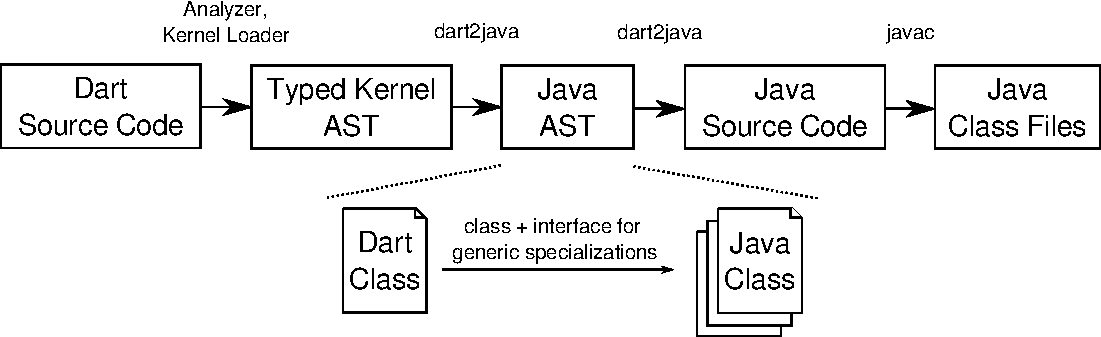
\includegraphics[width=\columnwidth]{dart2java_compile_user_code.pdf}
    \vspace{-10pt}
    \caption{Dart Code Compilation Process}
    \label{fig:user_code_compilation}
\end{figure}
dart2java uses \emph{Analyzer} and \emph{Kernel}\footnote{A front-end and an intermediate tree representation for Dart.} to generate a typed abstract syntax tree of every Dart class (Figure~\ref{fig:user_code_compilation}). This Dart AST is then transformed into a Java AST, generating one Java interface and one Java class for every Dart class, along with generic specializations (Section~\ref{sec:generic_spec}). The Java interface is necessary because every Dart class implicitly defines an interface that can be implemented by any class. The resulting Java source code can then be compiled and run with a copy of the compiled Dart SDK in the classpath.

The compilation process for the Dart SDK is mostly identical but starts with \emph{patching}: Some external methods are replaced with pure Dart implementations. For example, the external factory constructor\footnote{A factory constructor is a static method that is run when instantiating a class. It may return an instance of a subclass.} for \texttt{Map} is replaced with a concrete one, creating an instance of \texttt{LinkedHashMap}, a class that is implemented in Dart and shipped together with dart2java. Patching allows us to implement external methods in Dart without having to change the Dart SDK itself.

\begin{figure}[!tp]
\small
\begin{tabularx}{\columnwidth}{|l|X|}
\hline \hline
Constructor Semantics & Instance method for constructor body \\ \hline
Dynamic Type & Java Reflection/Method Handles API \\ \hline
Factory Constructors & Factory method is entry point for constructor \\ \hline
Getters / Setters & Java method prefixed with \texttt{get} / \texttt{set} \\ \hline
Generic Reification & First method/constr. arg.: \texttt{class<C>} object \\ \hline
Generic Covariance & Type safety ensured by runtime type system \\ \hline
Implicit Interfaces & Generate Java interface for Dart class \\ \hline
Keyword Parameters & Implicit \texttt{Map} object as last argument \\ \hline
Lambda Functions & Not supported yet \\ \hline
List / Map Literals & Special \texttt{List} / \texttt{Map} constructor with varargs \\ \hline
Mixins & Insert copy of mixin in hierarchy (fut. work) \\ \hline
\texttt{noSuchMethod} & Run handler if Java Reflection lookup fails \\ \hline
Operators & Ordinary Java method with name mangling \\ \hline
Optional Parameters & Automatically-generated method overloads \\ \hline
Synchronization & \texttt{async} / \texttt{await} are not supported yet \\ \hline
Top-level Members & Special \texttt{\_\_TopLevel\_\_} class \\ \hline
Type Casts & Runtime type system check (if necessary) and Java type cast \\
\hline \hline
\end{tabularx}
    \caption{Translation of Dart Language Features to Java}
        \vspace{-5pt}
    \label{fig:translation_overview}
\end{figure}
\begin{figure}[!tp]
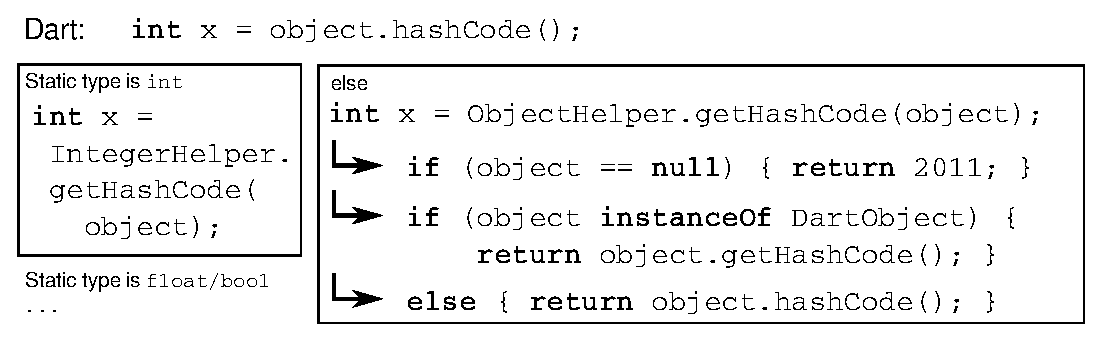
\includegraphics[width=\columnwidth]{helper_class.pdf}
    \vspace{-10pt}
    \caption{Method call with name defined in Dart \texttt{Object}}
    \vspace{-5pt}
    \label{fig:helper_object}
\end{figure}

\section{Code Generation}
This section describes the Java code generation process in dart2java (see Figure~\ref{fig:translation_overview} for an overview). The source code is already parsed and the type of every expression is known at this point of time.

\subsection{Datatypes}
There are a number of type checking modes in Dart. In \emph{unchecked mode}, all type names are treated as mere comments and actual types are inferred. dart2java is based on \emph{strong mode} which provides many type guarantees at compile time. Types can either be specified by the programmer or are inferred. Runtime type checking is required only for type casts, implicit downcasts and when assigning (or passing as an argument) an object whose type is generic.

Java provides boxed and unboxed versions for the primitive types \emph{boolean}, \emph{float}, \emph{double}, and \emph{integer}. dart2java always uses unboxed types, because they are significantly faster in numeric applications\footnote{Integers bigger than \texttt{Integer.MAX\_VALUE} are not supported.}. Method calls on such objects are translated to invocations of static methods of \emph{helper classes} (e.g., \texttt{IntegerHelper.gcd} for Dart \texttt{int.gcd}).  Calls to methods defined in Dart \texttt{Object} are dispatched to a primitive helper or to \texttt{ObjectHelper}, which can handle Dart objects, \texttt{null}, and ordinary Java objects outside of Dart's class hierarchy (Figure~\ref{fig:helper_object}). The generated Java code never uses boxed types except for the following cases.
\begin{itemize}
    \item Assignment (including passing arguments during method calls) to a variable (parameter) of type \texttt{Object} or \texttt{num}
    \item Generic class with $>2$ type parameters (Section~\ref{sec:generic_spec})
\end{itemize}

Every Dart class implicitly defines an interface that can be implemented by any other class. dart2java creates a class and an interface (interface names end with \texttt{\_IF}) for every Dart class and always uses the interface type during code generation except for instantiation of classes and invocation of static methods.

\paragraph{Class Hierarchy}
Dart supports single inheritance, interfaces and mixins. If no explicit superclass is specified, a Dart class is a subclass of \texttt{Object} (a core interface defined in the SDK). This interface provides the usual methods (e.g., for equality checking) and is implemented by the hand-written Java class \texttt{DartObject}, provided by dart2java. Every generated Java class implements exactly one interface: the interface that is generated for that class. If the corresponding Dart class implements other interfaces, the generated Java interface extends those interfaces. Mixins are future work.

\paragraph{Constructors}
Dart constructors are more powerful than Java constructors: There are ordinary constructors and \emph{factory constructors}, which are also invoked with the \texttt{new} keyword but are actually static methods (and can return existing objects) with a return type that can be any subtype of the class. Constructors can have names and classes can have multiple constructors. In addition, there is special special syntax for initializing fields (similar to C++), and a \texttt{super} constructor can be invoked at any point of time. For all constructors, the entry point in the generated Java code is a static method and the constructor body is in an instance method because Java constructors allow \texttt{super} calls only as the first statement.

\subsection{Non-nullability of Primitive Types}
One disadvantage of using unboxed types is that \texttt{null} can no longer be assigned to such variables. dart2java ships with a modified version of \emph{Analyzer} (the component performing type inference) to ensure that all variables of primitive type are explicitly initialized with a non-null value in the Dart user code. Casting a null value at runtime results in a null pointer exception. Moreover, dart2java's semantics of \texttt{Map} had to be changed. While the Dart SDK requires implementations to return \texttt{null} when looking up a non-existent key, our \texttt{Map} implementation throws an exception instead.

\subsection{Reified Generics}
In contrast to Java generics~\cite{Bracha:1998:MFS:286936.286957}, Dart generics are reified, i.e., an object knows the binding of its generic type variables at runtime (Java erases types). dart2java provides a runtime type system for checking types during assignments. Every Dart object has a field containing an object representing its (fully reified) type. Type checks are inserted when assigning/passing objects of generic type. 

\begin{lstlisting}
class A<T> {
  boolean isString() => T == String;
  void printToConsole(T item) { print(item); }
}
print(new A<String>().isString());
\end{lstlisting}
The generated Java class will have a \texttt{type} variable containing the reified type, which will be used for type checking. Furthermore, \texttt{printToConsole} will check if \texttt{item} is actually a string. 
\begin{lstlisting}
static final Type STR = /* ... */
static final Type A_STR = /* ... */

class A<T> implements A_IF<T> {
  private Type type;
  public A(Type type) {
    this.type = type; this._constructor();
  }
  boolean isString() {return type.typeParams[0] == STR;}
  void printToConsole(T item) {
    TypeSystem.check(item, type.typeParams[0]);
    System.out.println(item);
  }
}
System.out.println(new A<String>(A_STR));
\end{lstlisting}
Type checks for arguments of generic type have to be inserted due to generic covariance, as shown in the following listing. The Java type system alone cannot detect the type violation at runtime, because type information is erased.
\begin{lstlisting}
A<Object> a = new A<String>();
a.printToConsole(10);	// throw exception
\end{lstlisting}
Generic methods are also reified: An additional type object per type parameter will be passed as an argument.

\subsection{Covariant Generics}
In contrast to Java generics, Dart generics are covariant. Intuitively, covariance~\cite{Castagna:1995:CCC:203095.203096} means that subtyping takes into account the binding of generic type variables and requires them to be in a subtyping relationship as well. For example, \texttt{List<int>} is a subtype of \texttt{List<Object>} in Dart. Generated Java classes do not have to be generic. For example, a generic Dart class \texttt{A<T>} could be translated to a non-generic Java class \texttt{A} where all occurrences of \texttt{T} are replaced with \texttt{Object}. However, generated Java classes are generic for interoperability reasons (Section~\ref{sec:interop}): The generated code should be easy to use from Java without type casts. To make generated Java code compliant with the Java type system while preserving covariance, dart2java inserts casts to raw types. The following example defines a list of \texttt{A} and casts it to a list of \texttt{Object}, then to a list of \texttt{String}. This should trigger an exception at runtime.
\begin{lstlisting}
List<A> a = new List<A>();
List<Object> o = a;
// The following line causes a runtime error
List<String> s = o %*\textcolor{blue}{as}*) List<String>;
// Analyzer reports a (compile-time) error
List<String> s = a %*\textcolor{blue}{as}*) List<String>;
\end{lstlisting}
The generated Java code utilizes the runtime type system to perform type checks for downcasts.
\begin{lstlisting}
List_IF<A_IF> a = new List<A_IF>();
List_IF<Object_IF> o = (List_IF<Object_IF>)(List_IF) a;
// The following line causes a runtime error
List_IF<String> o = (List_IF<String>) (List_IF) 
    TypeSystem.check(a, LIST_STRING_TYPE);
\end{lstlisting}

\subsection{Generic Specializations}
\label{sec:generic_spec}
Using only unboxed versions of primitive types requires additional work when combined with generics, because Java allows only their boxed counterparts when used as generic types. dart2java could fall back to boxed types in such a case. However, since Dart does not have an array datatype and primitive types are widely used as generic types in many applications (typically with lists or maps), including in the benchmarks we used, dart2java generates specialized versions of generic classes for all primitive types.

For a generic class \texttt{A<T>}, dart2java generates four classes and interfaces. One class and interface is generated for each of \emph{bool} (\texttt{A\_\_bool}, \texttt{A\_\_bool\_IF)}, \emph{double} and \emph{int}. The fourth one (\texttt{A<T>},  \texttt{A\_IF<T>}) is a generic class/interface for all other types.

\begin{figure}[!htp]
	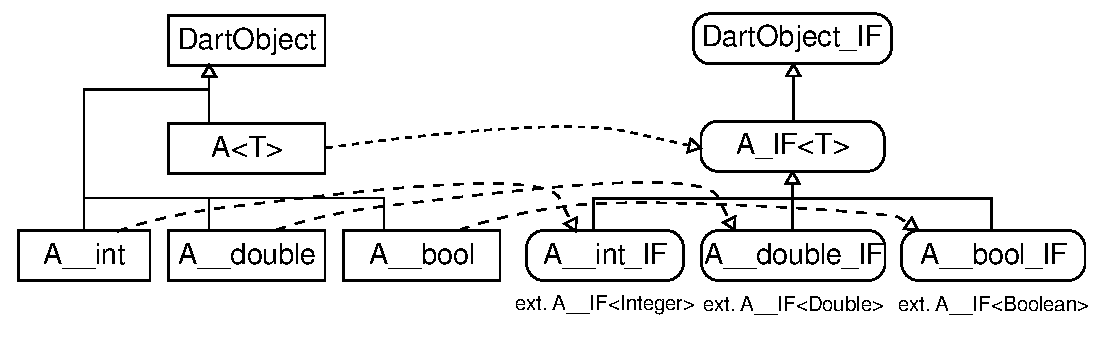
\includegraphics[width=\columnwidth]{generic_spec_classes.pdf}
    \vspace{-10pt}
    \caption{Generated Java Classes/Interfaces for \texttt{A<T>}}
    \label{fig:generic_spec_classes}
\end{figure}

Figure~\ref{fig:generic_spec_classes} illustrates the subclass relationship between those classes and interfaces. All generated classes are subclasses of \texttt{DartObject} (generated Java class for the Dart class \texttt{Object}) since no other superclass was specified. However, the specialized interfaces are subinterfaces of \texttt{A\_IF<T>}, where \texttt{T} is bound to the corresponding boxed type. This is necessary because of covariance (e.g., \texttt{A<int>} is a subtype of \texttt{A<Object>} in Dart). Inside a specialized class, all occurrences of \texttt{T} are replaced with the unboxed specialized type.

For classes with two generic type variables, all combinations of specializations are generated, i.e., 16 classes and 16 interfaces in total. No specializations are generated for classes with more than two type variables because of the combinatorial explosion of the number of classes, but annotations could be used to tell the compiler which types should be specialized for~\cite{Dragos:2009:CGT:1565824.1565830}.

dart2java's implementation class for the SDK interface \texttt{List<T>} is special: All of its specializations are hand-written and backed by a Java array. The implementation of \texttt{Map<K, V>} is written in Dart and backed by two Dart lists.

\begin{figure*}[!t]
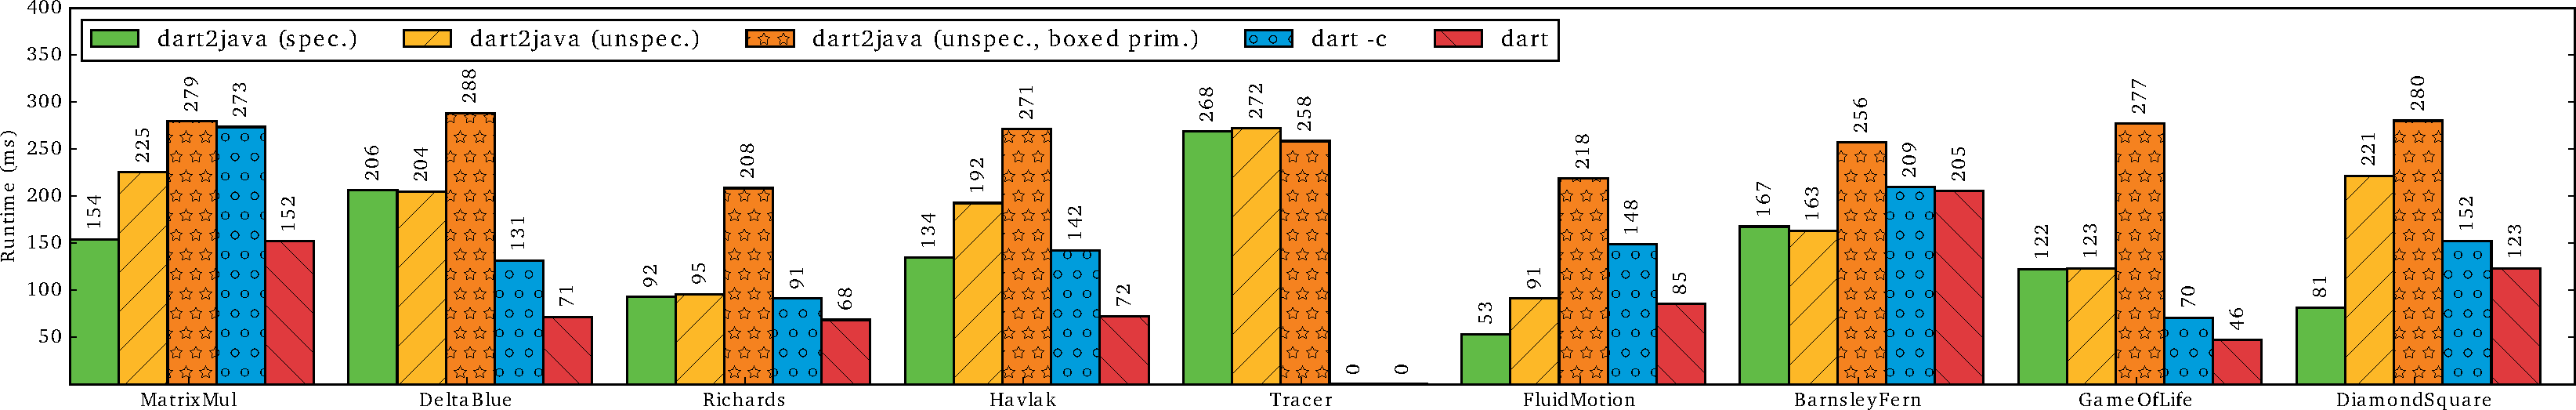
\includegraphics[width=\textwidth]{benchmark_plot.pdf}
\vspace{-10pt}
\caption{Benchmarks comparing dart2java (with/without specializations, with only boxed primitives) and Dart VM (checked/unchecked)}
\label{fig:benchmarks}
\end{figure*}

\subsection{Delegator Methods}
Unboxed primitive types are not subtypes of \texttt{Object} in Java. Therefore, overriding a method that consumes primitive types with a method consuming non-primitive types (or vice versa) requires additional effort. The problem is shown in its most basic form in the following Dart source code snippet.

\begin{lstlisting}
class A { void f(int a); }
class B extends A { void f(Object a); }
(new B()).f(10);
\end{lstlisting}

The generated Java source code would be mostly identical. However, \texttt{B.f} does not override \texttt{A.f}; instead, it defines a new method overload. The method call at the end of the snippet invokes the one defined in \texttt{A}. To solve this problem, dart2java adds \emph{delegator methods} for every method that consumes a primitive type but has a subtype where the method is overridden with one consuming a non-primitive type. Delegator methods perform a type cast and call the actual method, as shown below.

\begin{lstlisting}
void B.f(int a) { f((Integer) a); }
\end{lstlisting}

Delegator methods are also required for generic specializations. For example, for the method \texttt{List<T>.add(T obj)}, a delegator method \texttt{List\_\_int.add(Object obj)} is generated (delegating to \texttt{add(int obj)})\footnote{Our current implementation uses an unnecessarily more complex approach with name mangling, resulting in more delegator methods. However, the number of type casts and runtime method calls is identical.}.

The rule for generating delegator methods is as follows. Let us assume that we are translating \texttt{A.method}. Let $S$ be the set of all supertypes, i.e., super classes, interfaces, super interfaces and/or super types for generic type parameter bindings\footnote{For \texttt{Map<int, int>}, this includes \texttt{Map<Object, int>}, \texttt{Map<int, Object>} and \texttt{Map<Object, Object>}.}. For example, for \texttt{List<int>}, $S=\{\texttt{List<Object>}, \texttt{Object} \}$. For every $s \in S$, if \texttt{method} is defined in $s$ and \texttt{A.method} is not a valid Java override of \texttt{$s$.method}, generate a delegator method in \texttt{A} with the signature of \texttt{$s$.method}. A method is not a valid Java override if the types of the parameters are not identical/super types.


% List<Object> x = new List<int>();
% List<Object> x = new List__int();
% x.add(10);

\subsection{Benchmarks}
Figure~\ref{fig:benchmarks} shows the runtime of 9 benchmarks, comparing dart2java with the Dart VM. We ran the Dart VM in both checked mode and unchecked mode (the latter treats types as mere comments). dart2java is based on strong mode with additional compile-time type guarantees which is not available in the Dart VM yet, allowing us to avoid some runtime type checks (see Dart Language Guide). The Dart VM is the standard VM for Dart; ideally, dart2java should deliver performance comparable to the Dart VM. We ran all benchmarks on a system with an Intel Core i7-6820HQ CPU, 32 GB RAM, Ubuntu 16.04.1, OpenJDK 1.8.0\_111 and Dart VM 1.22.1.

Five benchmarks are taken from the ``ton80'' benchmark suite. Havlak uses a \texttt{Map<int, BasicBlock>} data structure, which is why the specialized version is faster here. The speedup is even better in FluidMotion, MatrixMul, DiamondSquare, which use \texttt{List<double>}, \texttt{List<List<int>>},  \texttt{List<List<int>>}, respectively. These three benchmarks along with BarnsleyFern (a highly numeric benchmark) are an indicator that the generated JVM code with unboxed primitive types can be executed faster on the JVM than on the Dart VM. However, some other benchmarks are slower in dart2java, mostly due to the overhead of instance creation and our runtime type system, which is not optimized for performance yet. In Tracer, all variables have type \emph{dynamic}. dart2java generates code that uses the Java Reflection API and the Java Method Handles API. It does not cache the method lookup results or perform any other optimizations~\cite{Marr:2015:ZMR:2737924.2737963}. The Dart VM can execute the same workload in less than one millisecond. Overall, the performance of dart2java is comparable to the Dart VM, even though the runtime type system is still unoptimized.

\section{Language Interoperability}
\label{sec:interop}
This section is mostly about future work. Some parts of our current implementation were designed with interoperability in mind, but more work has to be done.

\paragraph{Reusing Java Classes}
One main design decision is to reuse Java types as much as possible. For example, Dart \texttt{int} is mapped to Java \texttt{int} and our Java implementation of Dart \texttt{List<T>} does not only implement the interface that is generated from \texttt{List<T>} but also \texttt{java.util.List<T>}. Therefore, Dart lists can be passed to Java code and be used like normal Java lists. However, this is not sufficient yet. If a Dart method returns a Dart list, the return type will be \texttt{List\_IF<T>} or one of its specializations. This interface does not extend \texttt{java.util.List<T>}, but our Dart list implementation does. Therefore, programmers still have to manually cast such lists to Java's list interface. More crucially, user-defined Dart classes implementing Dart \texttt{List<T>} do not implement \texttt{java.util.List<T>}. To solve this issue, \texttt{List\_IF<T>} should extend \texttt{java.util.List<T>} and default interface methods should be added during SDK compilation, which implement the missing methods in terms of methods defined in Dart's list interface. The same technique can be applied to other Dart/Java interfaces such as \texttt{Map}, \texttt{Iterable} or \texttt{Iterator}. This technique fails if the Java and the Dart interface both define methods with the same name but different semantics. However, it seems that both languages are similar enough; the only (harmless) mismatch that we found was \texttt{List.add} which returns a boolean in Java but \texttt{void} in Dart.

\paragraph{Accessing Java Types in Dart}
It would be convenient if Dart programmers are able use Java classes and libraries in their code. Since \emph{Analyzer} performs type inference on Dart code, it requires some information about such Java classes. One high-level idea is to let programmers specify a Dart interface which is implemented by concrete Java classes. This is exactly how lists are implemented in dart2java. The interface \texttt{List<T>} is defined in the Dart SDK (therefore, \emph{Analyzer} can infer types) and the implementation class is written in Java. Interfaces could be generated automatically by a tool that analyzes all classes/interfaces of a library JAR file.

\paragraph{Generic Classes}
Generic classes in Java are not reified. Therefore, covariant downcasts on imported generic Java classes cannot be done in a safe way in Dart. This should trigger a warning. If Java programmers want to use a Dart class, they have to provide the reified type as an additional argument to the constructor. Since the generated Java classes also use Java generics, the Java interface has proper types (and not just \texttt{Object} for generic types).


\section{Related Work}
There are two main techniques for language interoperability: source-to-source compilation (e.g., dart2java, DDC, TypeScript) and multi-language virtual machines~\cite{multivm_saarlang, vranythesis}. If the languages are similar enough (like in dart2java), the methods and objects from the other language can directly be used without naming or semantics conflicts. Otherwise, proxy/adapter objects/interfaces~\cite{DBLP:journals/jot/EkmanMS07}, name mangling or different method calling notations~\cite{DBLP:journals/corr/Springer16} must be used. 

dart2java generates all specialized versions for classes with up to two type variables. Alternatively, specializations could be generated when used~\cite{Kennedy:2001:DIG:378795.378797}, possibly using JIT compilation, or specialization could be guided by annotations~\cite{Dragos:2009:CGT:1565824.1565830}. In general, code with reified generics can executed more efficiently than code with unreified generics, because more information is known at runtime. For example, \texttt{List<String>[i]} always is guaranteed to always return a string. In Java's case, a list of integers could masquerade as a list of strings using unsafe type casts. Therefore, Java has to add additional type casts~\cite{Nino:2007:CEJ:1229688.1229690, BrachaJuly52004}. Because dart2java emits Java code (and not bytecode) and specializations are generated only for primitive types, the resulting Java bytecode contains such (redundant) type checks, even though our runtime type system already ensures type safety (list of integers cannot masquerade as list of strings). C\# has reified generics and avoids such redundant type checks~\cite{Kennedy:2001:DIG:378795.378797}.


\section{Conclusion}
We presented dart2java, a source-to-source compiler which allows programmers to run Dart code on the JVM.  Due to their similarities, we think that Dart is a good fit for the JVM if performance considerations are taken into account. As our benchmarks show, dart2java's performance is comparable to the Dart VM's performance. Interoperability between Dart and Java is still limited at this point of time and subject to future work.

\begin{acks} 
We would like to thank Vijay Menon, Jennifer Messerly and Leaf Peterson from Google Seattle for their guidance and mentorship while working on this project. 
\end{acks}

% The 'abbrvnat' bibliography style is recommended.

% The bibliography should be embedded for final submission.

\bibliographystyle{plain}
\bibliography{icooolps2017}

\appendix
\section{Appendix: Full Example}
The following listing shows a generic class in Dart code. It also  illustrates examples of where Dart syntax is different from Java syntax, such as getters and named constructors.

\begin{lstlisting}
class MyMap<K, V> extends Map<K, V> {
  List<K> keys;
  List<V> values;

  int get size => keys.length;
  bool get isEmpty => keys.isEmpty;

  MyMap() {
    keys = new List<K>();
    values = new List<V>();
  }

  MyMap.fromList(List<K> keys, List<V> values) : keys = keys, values = values;

  V operator [](K key) {
    for (int i = 0; i < keys.length; i++) {
      if (keys[i] == key) {
        return values[i];
      }
    }

    throw "Key not found";
  }
}
\end{lstlisting}

The following listing shows the generated Java class (without specializations and interfaces).

\begin{lstlisting}
class MyMap<K, V> extends DartObject implements MyMap_IF<K, V> {
  dart.core.List_IF<K> keys;
  dart.core.List_IF<V> values;

  int getSize() { return keys.getLength(); }
  boolean getIsEmpty() { return keys.getIsEmpty(); }
  
  public MyMap(Type type) {
    this.type = type;
  }
  
  public static <K, V> MyMap_IF<K, V> new_(Type type) {
  	MyMap_IF<K, V> instance;
   
    if (type.typeParams[0] == INT_TYPE && type.typeParams[1] == INT_TYPE) {
      instance = new MyMap__int_int(type);
    } else if (/* ... */) { /* ... */
    } else {
      instance = new MyMap<K, V>(type);
    }
    
    instance._constructor();
    return instance;
  }
  
  public static <K, V> MyMap_IF<K, V> new_fromList(Type type, List_IF<K> keys, List_IF<V> values) {
  	MyMap_IF instance;
    // (Initialize instance)
    
    instance._constructor_fromList(keys, values);
    return instance;
  }
  
  public V operatorAt_MyMap(K key) {
    for (int i = 0; i < getKeys().getLength(); i++) {
      if (dart._runtime.helpers.ObjectHelper.operatorEqual(getKeys().operatorAt(i), key)) {
        return getValues().operatorAt(i);
      }
    }
    throw new RuntimeException("Key not found");
  }
}
\end{lstlisting}

\section{Links to Dart Components}
\begin{itemize}
	\item dart2java: \url{https://github.com/google/dart2java} \\
    This repository also contains all the benchmarks used in this paper and the generated Java source code.
	\item Dart Analyzer:\\ \url{https://pub.dartlang.org/packages/analyzer}
    \item Kernel: \url{https://github.com/dart-lang/kernel}
    \item Dart to JavaScript Compiler (DDC): \url{https://github.com/dart-lang/sdk/tree/master/sdk/lib/js/dart2js}
    \item Dart Language Guide, strong mode: \\ \url{https://www.dartlang.org/guides/language/sound-dart}
\end{itemize}
\end{document}
